\documentclass[11pt,a4paper]{report}
\usepackage[margin=1in]{geometry}
\usepackage[japanese]{babel}
\usepackage{datetime2}
\usepackage{titlesec}
\usepackage{tocloft}
\usepackage{amsmath}
\usepackage{indentfirst}
\usepackage{fancyhdr}
\usepackage[dvipdfmx]{graphicx}

\newcommand{\Writer}[1]{
  \normalsize
  \begin{flushright}
    (※文責:#1)
  \end{flushright}
}
\newcommand{\AgendaBox}[2]{
    \large
    \textbf{#1}\\

    \vspace{0.2cm}

    \small 
    #2

    \vspace{0.5cm}
}
\newcommand{\NameBox}[2]{
    \small 
    #1\hspace{1cm}#2
}
% Chapter title formatting
\titleformat{\chapter}[hang]
  {\bfseries\huge} % Title style
  {第 \thechapter 章} % Label
  {1em} % Spacing between label and title
  {\huge} % Title font
% Section title formatting
\titleformat{\section}{\LARGE\bfseries}{\arabic{chapter}.\arabic{section}}{1em}{}
\titleformat{\subsection}{\large\bfseries}{\thesubsection}{1em}{}
\renewcommand{\thesubsection}{\normalsize\arabic{chapter}.\arabic{section}.\arabic{subsection}}

% ヘッダーとフッターをカスタマイズ
\fancyhead{} % 既存のヘッダーをクリア
\fancyfoot{} % 既存のフッターをクリア
\fancyfoot[C]{\thepage} % フッター中央にページ番号を表示

\begin{document}
\thispagestyle{empty}
\begin{center}
    \large
    \textbf{
      公立はこだて未来大学 2024年度 システム情報科学実習\\
      グループ報告書
    }\\

    \vspace{0.2cm}

    \small 
    \textbf{
      Future University Hakodate 2024 Systems Information Science Practice\\Group Report
    }

    \vspace{0.5cm}

    \AgendaBox{プロジェクト名}{境界なく人々の生活を支援する技術}
    \AgendaBox{Project Name}{DLITE3 : Technology that supports people's lives without boundaries}
    \AgendaBox{グループ名}{自然エンタメ班 班}
    \AgendaBox{Group Name}{Nature Entertainment Gropu}
    \AgendaBox{プロジェクト番号 / Project No.}{22}
    \AgendaBox{プロジェクトリーダ / Project Leader}{金子康一\hspace{1cm}Kaneko Koichi}
    \AgendaBox{グループリーダー / Group Leader}{
      \NameBox{伊丸岡朝陽}{Imaruoka Asahi}\\
    }
    \AgendaBox{グループメンバー / Group Member}{
      \NameBox{金子康一}{Kaneko Koichi}\\
      \NameBox{伊丸岡朝陽}{Imaruoka Asahi}\\
    }
    \AgendaBox{指導教員}{
      三上貞芳 伊藤精英 宮本エジソン正 島影圭佑
    }
    \AgendaBox{Advisor}{
      Mikami Sadayoshi Ito Kiyohide Miyamoto, Edson T. Shimakage Keisuke
    }
    \AgendaBox{提出日 / Date of Submission}{
      2024年7月12日 July 12, 2024
    }
    

\end{center}

% 空のページを挿入
\newpage
\thispagestyle{empty}
\mbox{}
\newpage

\clearpage
\pagenumbering{arabic}
\setcounter{page}{1}

{
    \centerline{
      \huge\textgt{概要}
    }
    \vspace{1cm}
    \noindent\space
    本プロジェクトでは、「視覚や聴覚に頼れない状況で役立つ装置の開発」をコンセプトとし、障がい者が抱える問題を当事者目線で
検討し、実用的な装置の開発に取り組んできた。頼れない感覚を別の手段で補うことで、不便を解消し、安全で快適な生活を支援す
ることを目指している。聴覚障がいや視覚障がい、色覚の障がい者を対象とした4つのグループに分かれ、それぞれ、特定の言葉や
音に反応するデバイス、画像の色をユニバーサルデザインに変換するアプリ、自力で避難することが難しい人のための補助デバイ
ス、障がい者が自然を楽しむためのデバイスの開発を行っている。

}
\newpage
{
    \centerline{
      \textbf{\huge\textgt{Abstract}}
    }
    \vspace{1cm}
    \noindent\space
    Under the concept of "developing devices that are useful in situations where one cannot rely on sight or hearing," this project examines the
problems faced by people with disabilities from the perspective of the people concerned, to develop practical devices. By supplementing
unreliable senses with other means, the project aims to eliminate inconvenience and support safe and comfortable living. The project is
divided into four team targeting people with hearing disabilities, visual disabilities, and color blindness. Each team is developing devices that
respond to specific words and sounds, applications that convert the color of images to universal design, assistive devices for people who
have difficulty evacuating on their own, and devices that allow people with disabilities to enjoy nature.

}
\newpage

% Table of contents (optional)
\tableofcontents
\newpage

% 本文ページ
\chapter{はじめに}
\section{背景}
\noindent\space
普段の日常生活では木々や空、風の音など様々な自然に触れる機会があり、無意識のうちに楽しんでいると考える。
しかし、視覚や聴覚に障がいを持つ人は自然の音を聞くことや景色を見ることが難しい。
それにより、自然を最大限楽しむことが出来ないと考える。
\Writer{金子康一}

\section{先行研究}
\noindent\space
峰野は視覚障害者が散策する目的として、気候や季節を見計らって気分転換がてらに行う要因があると述べている(峰野 2013)。しかし視覚障がい者は目での観察が不可能なため、気分転換の効果が軽減してしまうのではないかと考える。これは音を聞くことが出来ない聴覚障がい者にも言えるのではないかと考えた。
\Writer{伊丸岡朝陽}

\section{研究動機}
\noindent\space
私たちのグループでは、まずフィールドワークから行った。
フィールドワークの内容は以下の2つを室内、屋外で行った。
% フィールドワークの内容
\begin{enumerate}
  \item イヤフォンで耳を塞いだ状態で外部の音を完全に遮断し徘徊する。
  \begin{itemize}\item[-] 聴覚情報の遮断\end{itemize}
  \item 5分間目を瞑った状態で座る。
  \begin{itemize}\item[-] 視覚情報の遮断\end{itemize}
\end{enumerate}
その結果、以下のことに気付いた。
% フィールドワークの結果
\begin{itemize}
  % ===== 聴覚 =====
  \item 聴覚情報の遮断
  \begin{itemize}
    \item 室内
    \begin{itemize}
      \item 一緒に歩いている人の足音が聞こえないため、視界から外れたときに足音が聞こえなくてついてきているのか分からない。
      \item 曲がり角や階段の頂上付近で人が来ているのか足音から分からず、普段より警戒した。
      \item 自分のコツコツとした足音が聞こえず、歩いている感がない。
    \end{itemize}
    \item 屋外
    \begin{itemize}
      \item 風の音や風が吹くことによる音(葉っぱが揺らぐ音など)が聞こえず、涼しさや季節感を感じられにくかった。
      \item 芝生を歩いたが、コンクリートよりも歩いたときの感触が強いので、歩いているという感覚が強い。
      \item 道路を渡る時に車が来ているのか音での判別ができず若干危険。
    \end{itemize}
  \end{itemize}
  % ===== 視覚 =====
  \item 視覚情報の遮断
  \begin{itemize}
    \item 室内
    \begin{itemize}
      \item 会話をする中で説明をする際にジェスチャーが使えなくて不便。
      \item 音に集中するため音の聞こえ方がより立体的になる。
      \item 会話のとき、ジェスチャーが使えないので簡単な「上」や「下」を使って説明することがあった。
    \end{itemize}
    \item 屋外
    \begin{itemize}
      \item 花の色が見れない。
      \item 木々の揺れ方は音からある程度は伝わるがどの程度揺れいているのかのイメージがつかみにくい。
      \item 日が昇っているのか沈んでいるのか分からない。
    \end{itemize}
  \end{itemize}
\end{itemize}
これらの結果から、室内では危険が増えることが分かった。
また屋外では、危険が増えるだけでなく、日常的に触れている自然が感じられにくくなった。
これらを踏まえ、障がいの有無に関わらず、自然を楽しむことが出来るようにしたいと感じた。
\Writer{金子康一}

\section{目的}
\noindent\space
本プロジェクトでは、視覚、聴覚の障がいの有無に関わらず、自然を楽しむことのできる「自然エンタテインメントデバイス」を開発し、自然の新たな楽しみ方を実現したい。
\Writer{金子康一}

\chapter{関連研究}
\section{使用技術}
\noindent\space
hogehoge
\Writer{金子康一}

\section{解決手法}
\subsection{サブセクション1}
\noindent
hogehoge
\Writer{金子康一}

\subsection{サブセクション2}
\noindent
hogehoge
\Writer{金子康一}

\chapter{活動の要約}
\section{成果}
\noindent\space
\subsection{使用技術}
\begin{center}
  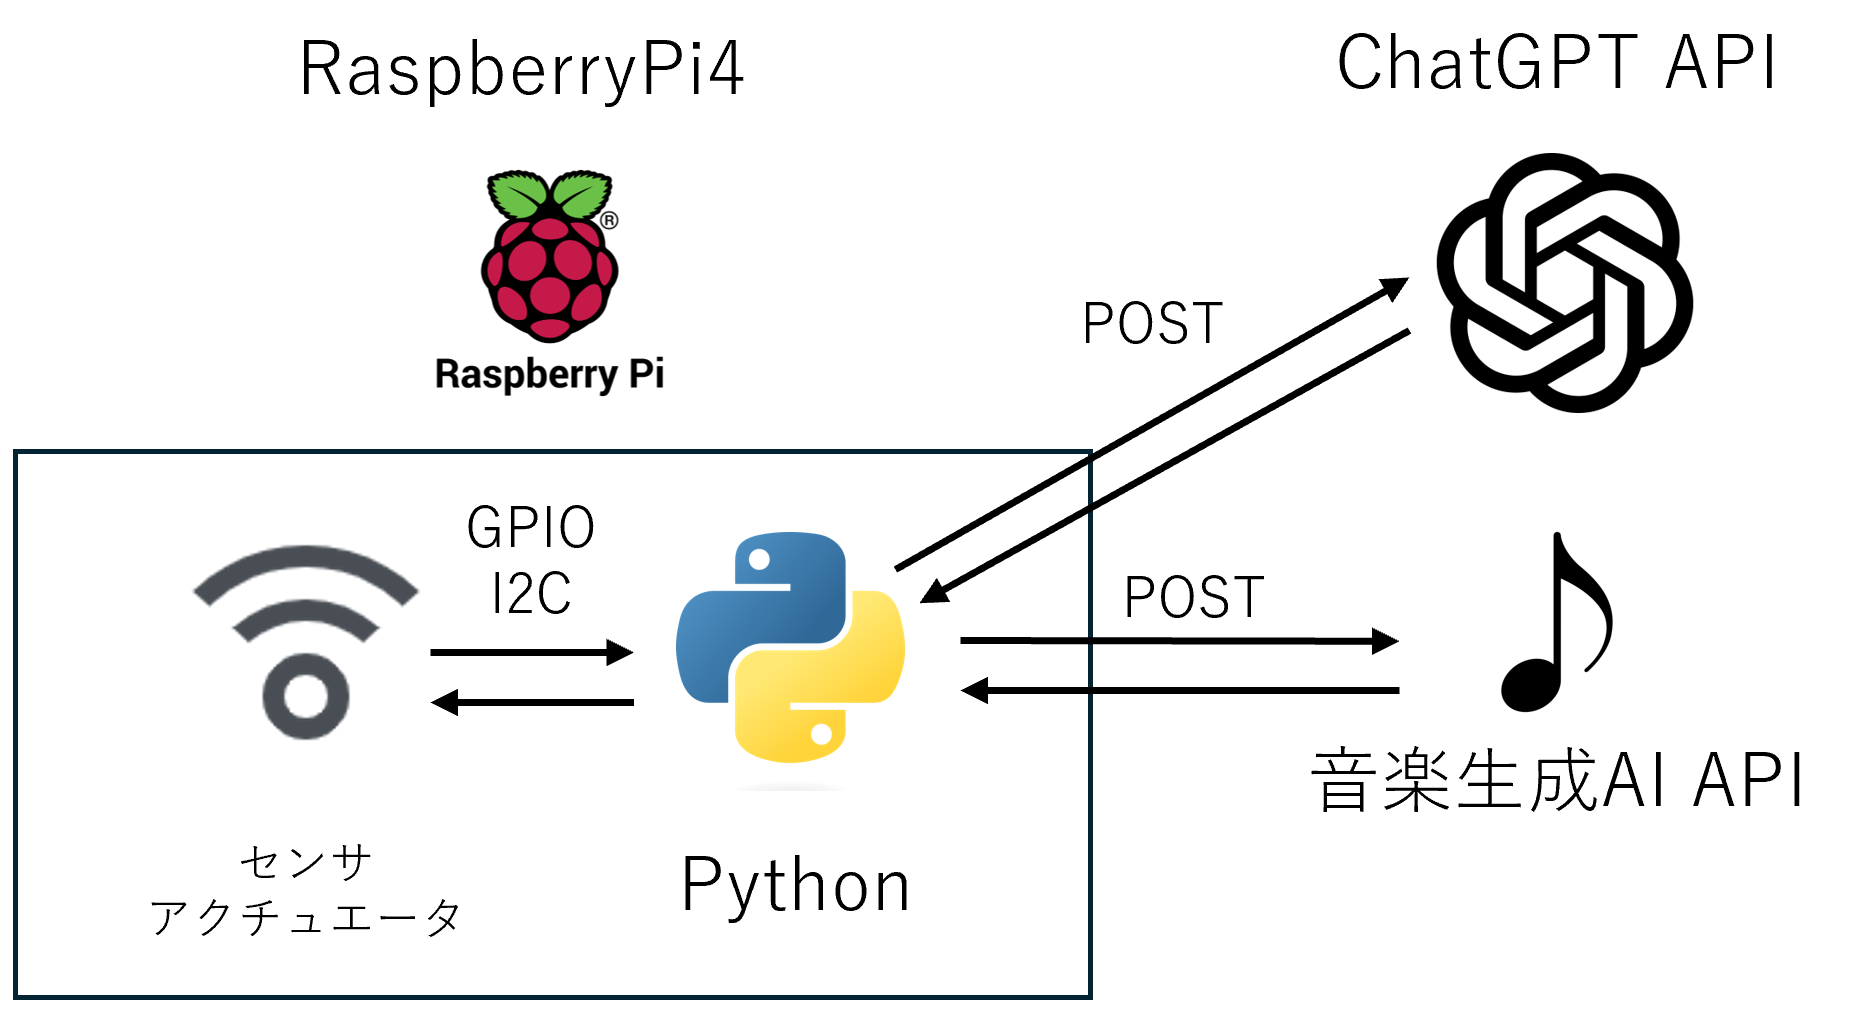
\includegraphics[width=100mm]{images/tech-conf.png}\\
  図1  :技術構成
\end{center}
\Writer{金子康一}

\section{活動計画}\noindent
\subsection{開発環境}
\Writer{金子康一}

\subsection{ハードウェア}
\Writer{金子康一}

\subsection{ソフトウェア}
\Writer{伊丸岡朝陽}

\end{document}
